\section{MOS Transistoren}

\subsection{Dotierung}
\begin{center}
    \begin{tabular}{lll}
        \textbf{Dotierung:}          & N-dotiert            & P-dotiert \\
        \textbf{Unreinheit:}         & Aluminium (HG III)   & Phosphor / Arsen (HG V) \\
        \textbf{Majoritätsträger:}   & Elektronen           & Löcher \\
        \textbf{Minoritätsträger:}   & Löcher               & Elektronen \\
    \end{tabular}
\end{center}


\subsection{MOS-Kapazität}
\begin{minipage}[t]{0.5\columnwidth}
    Minoritätsträger werden an das Gate gezogen.
    Die entstandene Raumladungszone weist bei ausreichend hoher Gate-Spannung einen Minoritätsträgerüberschuss auf, ist also in der Funktion \textbf{komplementär} zum Substrat dotiert.
\end{minipage}
\hfill
\begin{minipage}[t]{0.48\columnwidth}
    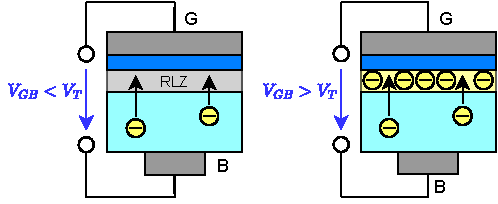
\includegraphics[width=\columnwidth, align=t]{images/MOS_kapazitaet.pdf}
\end{minipage}


\subsection{MOS-Transistoren}
Werden links und rechts vom MOS-Kondensator komplementär zum Substrat dotierte Regionen (Drain und Source) erstellt, so kann ohne Gatespannung aufgrund der PN-Übergänge kein Strom vom Drain zur Source (oder umgekehrt) fliessen.
Wird nun eine Spannung am Gate angelegt, so entsteht die Minoritätsträger-Leitende Raumladungszone - der Kanal.
Dieser verbindet Drain und Source, es kann also ein Strom fliessen.

\vspace{-0.2cm}

\begin{center}
    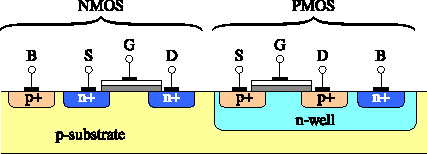
\includegraphics[width=0.5\columnwidth, align=t]{images/01_CMOS.pdf}
\end{center}


\subsubsection{Übersicht und Symbole}

\begin{minipage}[t]{0.48\columnwidth}
    Durch Vordotierung des Kanals kann der Transistor ohne Gate-Spannung leitend gemacht werden (Verarmungstyp, selbstleitend).
    Eine negative Gate-Spannung kann den Kanal dann abschnüren. Verarmungstypen werden in dieser Vorlesung nicht behandelt.

    \smallskip

    Der Bulk wird nur eingezeichnet, wenn dieser nicht mit der Source verbunden ist.
    Deshalb werden meist die vereinfachten Symbole verwendet.

    \vspace{-0.3cm}

    \begin{center}
        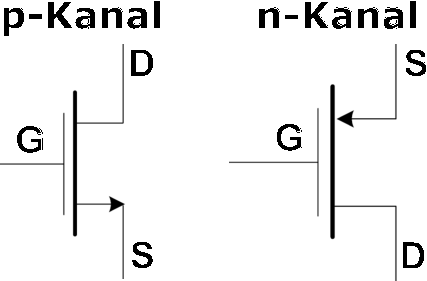
\includegraphics[width=0.45\columnwidth, align=t]{images/MOSFET_symbole_vereinfacht.pdf}
    \end{center}
\end{minipage}
\hfill
\begin{minipage}[t]{0.5\columnwidth}
    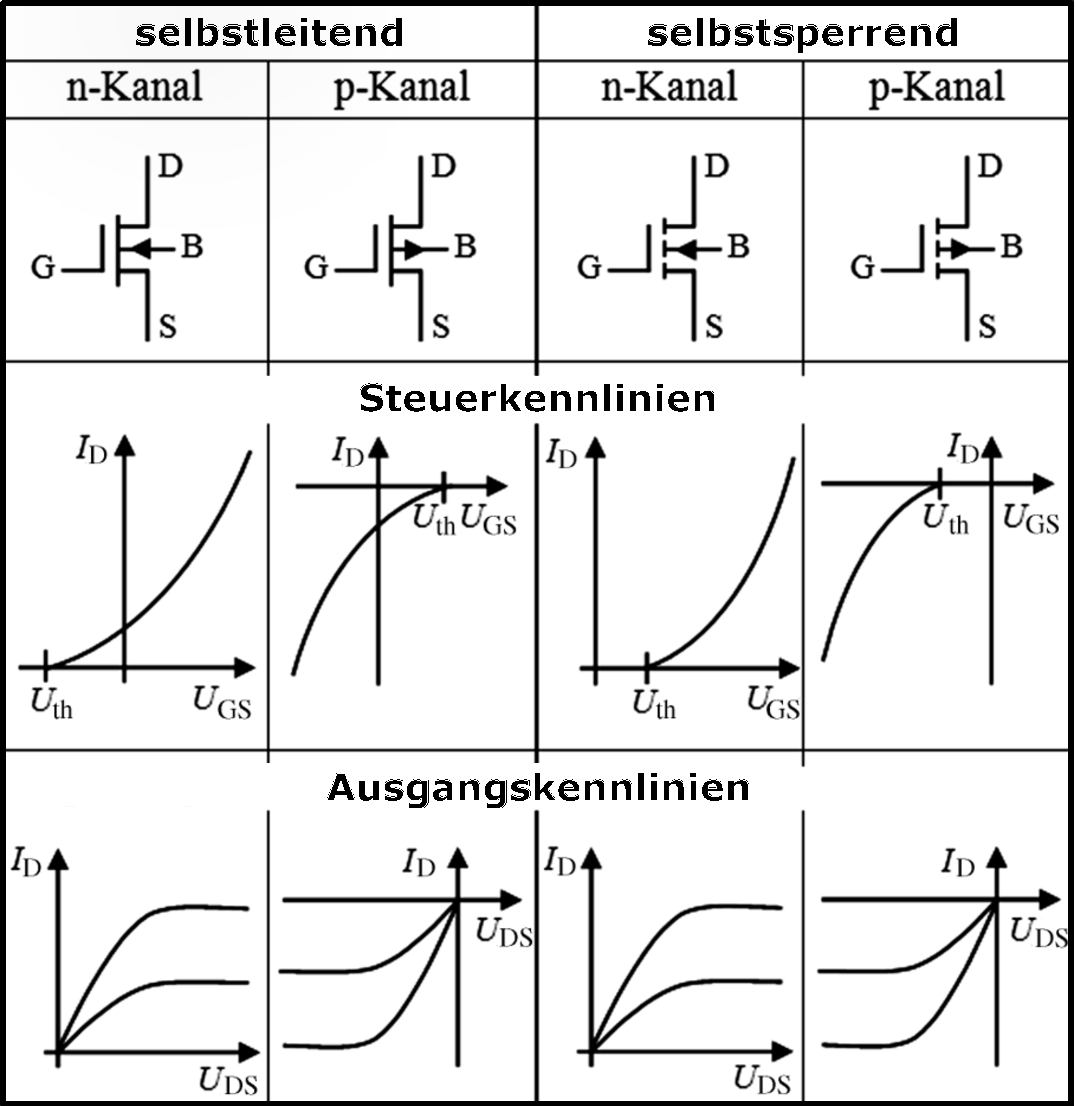
\includegraphics[width=\columnwidth, align=t]{images/MOSFET_uebersicht.pdf}
\end{minipage}



\subsubsection{Modelle}
In Cadence sind verschiedene Modelle hinterlegt:

\textbf{Spice Modell 11:} Das Modell 11 beinhaltet ca. 100 Parameter und ist entsprechend genau.

\textbf{Spice Modell 1:} Vergleichbar mit dem Handrechenmodell, welches zwar weniger genau, dafür aber viel einfacher ist. Dennoch beinhaltet es bereits 40 Parameter.

\subsection{Ausgangskennlinie -- Arbeitsbereiche}
 
Die Ausgangskennlinie beschreibt den Zusammenhang $I_D = f(V_{DS}) \big|_{V_{GS} = \text{konst}}$

\begin{minipage}[t]{0.5\columnwidth}
    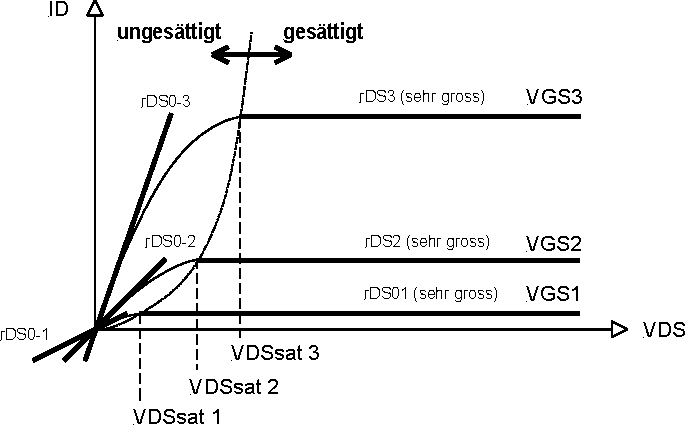
\includegraphics[width=\columnwidth, align=t]{images/MOSFET_ausgangskennlinien.pdf}
\end{minipage}
\hfill
\begin{minipage}[t]{0.48\columnwidth}
    Zwei Arbeitsbereiche: 

    \begin{outline}
        \1 ungesättig (gesteuerter Widerstand)
        \1 gesättigt (Stromquelle)
    \end{outline}

    \medskip

    Die Sättigungsgrenze $V_{\rm DS, sat}$ ist abhängig vom \textbf{Kanalzustand}:

    \begin{outline}
        \1 \textbf{weak inversion:} \\
            $V_{\rm DS, sat} = V_{\rm eff} \approx 5 \cdot V_{\rm temp} \approx \qty{130}{\milli \volt}$ 
        \1 \textbf{strong inversion:} \\
            $V_{\rm DS, sat} = V_{\rm eff} = V_{GS} - V_T$ 
    \end{outline}
\end{minipage}



\subsection{Transferkennlinie -- Ausgangsstrombereiche}


\begin{minipage}[t]{0.55\columnwidth}
    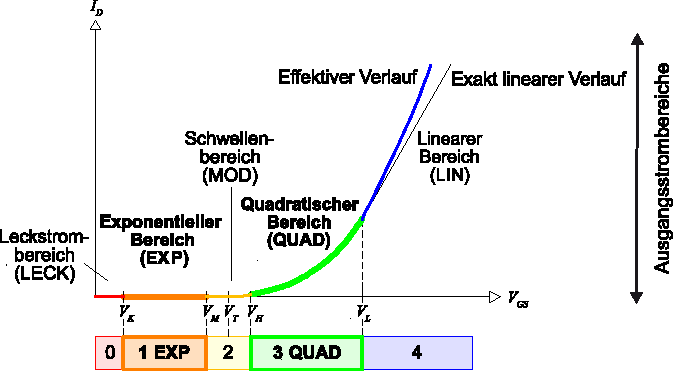
\includegraphics[width=\columnwidth, align=t]{images/MOSFET_transferkennlinie.pdf}
\end{minipage}
\hfill
\begin{minipage}[t]{0.42\columnwidth}
    Die Transferkennlinie beschreibt den Zusammenhang $I_D = f(V_{GS})$ 

    \smallskip

    Dabei werden \textbf{5 Ausgangsstombereiche} unterschieden. Diese hängen mit dem \textbf{Kanalzustand} zusammen.

    \smallskip

    Des Weiteren gibt es die Bereiche:

    \begin{outline}
        \1 Subthreshold: $V_{GS} < V_T$
        \1 Above Threshold: $V_{GS} > V_T$
    \end{outline}
\end{minipage}


\para{Ausgangsstrombereiche}

\scalebox{0.8}{
\begin{tabular}{|l|l|l|}
    \hline
    \textbf{Bereich}                    & \textbf{Mathem. Charakterisierung}            & \textbf{Zugrundeliegender phys. Effekt}                       \\  
    \hline
    \rowcolor[HTML]{F4CCCC} 
    LECK                                & $I_D$ erreicht Minimalwert, der nicht         & Drain- und Source-Substratdiode haben                         \\
    \rowcolor[HTML]{F4CCCC} 
                                        & weiter unterschritten werden kann             & Leckströme ins Subsstrat                                      \\
    \hline
    \rowcolor[HTML]{FFE5BB} 
    EXP                                 & $I_D$ steigt exponentiell mit $V_{GS}$        & Kanal zeigt \textbf{weak inversion}                           \\
    \hline
    \rowcolor[HTML]{FFF2CC} 
    MOD                                 & Keine 'handliche' Formel für $I_D$            & Kanal zeigt \textbf{moderate inversion}                       \\
    \hline
    \rowcolor[HTML]{D9EAD3} 
    QUAD                                & $I_D$ steigt quadratisch mit $V_{GS}$         & Kanal zeigt \textbf{strong inversion}                         \\
    \hline
    \rowcolor[HTML]{CFE2F3} 
    LIN                                 & $I_D$ steigt annähernd linear mit $V_{GS}$    & Geschwindigkeitssättigung der Ladungsträger im Kanal          \\
    \rowcolor[HTML]{CFE2F3} 
                                        & (halb QUAD, halb LIN)                         & im Kanal (nicht weiter beschleunigbar)                        \\
    \hline
\end{tabular}
}

\smallskip

\textbf{Hinweis:} Die Inversion des Kanals beschreibt, wie sehr sich die Polarität geändert ('invertiert') hat. 
Bei einem n-Kanal FET ist der Kanal ursprünglich p-leidend.
Wird der Kanal invertiert, so wird er (schwach, moderat oder start) n-leitend. 


\subsection{Ersatzschaltungen}

Je nach Arbeitsbereich (gesättigt / ungesättigt) müssen verschiedene Ersatzschaltungen verwendet werden.

\begin{minipage}[t]{0.48\columnwidth}
    \raggedright

    \subsubsection*{Ungesättigt}

    Gesteuerter Widerstand \rightarrow\ $I_D = f(V_{DS})$
    
    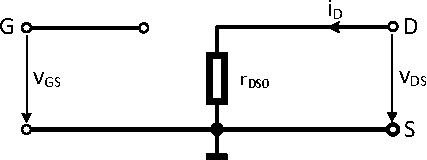
\includegraphics[width=\columnwidth, align=t]{images/MOSFET_ersatzschaltung_ungesaettigt.pdf}

    \smallskip
    Je kleiner $r_{\rm DS0}$, desto steiler die Geraden links im Ausgangskennlinienfeld

\end{minipage}
\hfill
\begin{minipage}[t]{0.48\columnwidth}
    \raggedright

    \subsubsection*{Gesättigt}

    Stromquelle \rightarrow\ $I_D = f(V_{GS})$

    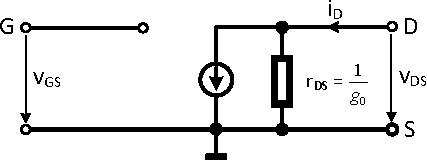
\includegraphics[width=\columnwidth, align=t]{images/MOSFET_ersatzschaltung_gesaettigt.pdf}

    \smallskip
    Je grösser $r_{\rm DS}$, desto flacher die Geraden rechts im Ausgangskennlinienfeld
\end{minipage}


\subsection{Berechnung des Drainstroms}

% CHECK [Simi] @Flurin (gnaze subsection): Formeln für p-Kanal UND n-Kanal? (im Skript ist beides, in den Slides nicht)
% CHECK [Simi] @Flurin (gnaze subsection): Kanallängenmodulation Faktor $(1 + \lambda)$ bei Formeln hinzufügen? (ist im Skript enthalten, in den Slides nicht)

Die Berechnung des Drainstroms hängt sowohl von Arbeitsbereich (gesättigt / ungesättig), als auch vom Ausgangsstrombereich (bzw. der Kanaliversion) ab!


\subsubsection{Strong Inversion}

\vspace{-0.3cm}

$$ \boxed{ \text{QUAD-Bereich: } V_H(I_D) < V_{GS} < V_L(I_D) } \qquad \qquad \beta = \mu \cdot C_{\text{OX}} \cdot \frac{W}{L} $$


\renewcommand{\arraystretch}{1.5}
\begin{ctabular}{c|c}
    \textbf{Ungesättigt}                                                            & \textbf{Gesättigt}                        \\
    $I_D = \beta \cdot \bigg[ (V_{GS} - V_T) V_{DS} - \frac{V_{DS}^2}{2} \bigg]$    & $I_D = \frac{\beta}{2} (V_{GS} - V_T)^2$
\end{ctabular}
\renewcommand{\arraystretch}{1}



\subsubsection{Weak Inversion}

\vspace{-0.3cm}

$$ \boxed{ \text{EXP-Bereich: } V_K(I_D) < V_{GS} < V_M(I_D) \qquad \qquad V_M(I_D) = V_T(I_D) - x_M(I_D) } $$

%TODO bzw CHECK [Simi] @Flurin Vtemp Formel auch irgendwo ergänzen? Wert für Vtemp in Übungen immer aus Technologiehandbuch gegeben
% $V_{\rm temp} = \frac{kT}{q}$
% $k$: Boltzmann-Konstante
% $q$: Elementarladung
% $T$: Temperatur in Kelvin

\renewcommand{\arraystretch}{1.5}
\begin{ctabular}{c|c}
    \textbf{Ungesättigt}                                                                                                & \textbf{Gesättigt}                                                    \\
    $I_D = I_M \cdot \e^{\frac{V_{GS} - V_M}{n_M \cdot V_\text{temp}}} \cdot (1 - \e^{-\frac{V_{DS}}{V_\text{temp}}})$  & $I_D = I_M \cdot \e^{\frac{V_{GS} - V_M}{n_M \cdot V_\text{temp}}}$
\end{ctabular}
\renewcommand{\arraystretch}{1}


\subsubsection{Bereiche ohne Berechnungsformeln}

In den drei verbleibenden Bereichen sind \textbf{keine Berechnungsformeln für} $\bm{I_D}$ vorhanden.

\smallskip

\begin{minipage}[c]{0.48\columnwidth}
    \renewcommand{\arraystretch}{1.2}
    \begin{ctabular}{lll}
        \textbf{Bereich}    & \textbf{Grenzen}                  \\
        LECK                & $V_K(I_D) < V_{GS} < V_M(I_D)$    \\ 
        MOD                 & $V_M(I_D) < V_{GS} < V_H(I_D)$    \\ 
                            & $V_H(I_D) = V_T(I_D) + x_H(I_D)$  \\
        LIN                 & $V_L(I_D) < V_{GS}$               \\ 
    \end{ctabular}
\end{minipage}
\hfill
\begin{minipage}[c]{0.48\columnwidth}
    Im MOD-Bereich (moderate inversion) liefern die Formeln der weak bzw. strong inversion katastrophal falsche Resultate!

    \smallskip

    Es ist daher enorm wichtig, den Arbeitsbereich des Transistors korrekt zu bestimmen.
\end{minipage}
